% !TEX root = main.tex

\section{表示与描述} % Chap 11
图像表示与描述有两种方法:
\begin{itemize}
	\item 外部描述:形状
	\item 内部描述:颜色与纹理
\end{itemize}

\subsection{表示方法}
\subsubsection{链码}
链码用于表示由顺次连接的具有指定长度和方向的直线段组成的边界线

链码种类:4向链码和8向链码
\begin{figure}[H]
\centering
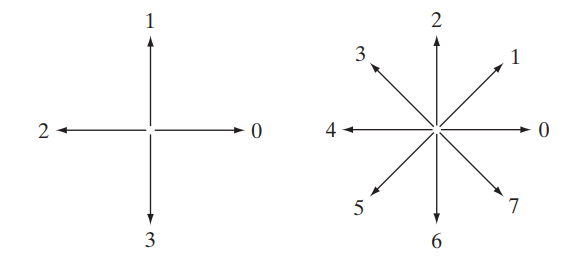
\includegraphics[width=0.4\linewidth]{fig/chain_code.png}
\end{figure}

常见的问题:
\begin{enumerate}
\item 得到的链码太长;
\item 噪声或边界缺陷的影响;
\end{enumerate}

解决方案:选择更大间隔的网格对边界进行重新采样。
\begin{itemize}
\item 边界链码依赖于起始点(通过归一化可一致,即使链码最小)
\item 用差分码(逆时针旋转的方向数)可以将链码旋转归一化
\end{itemize}
\begin{figure}[H]
\centering
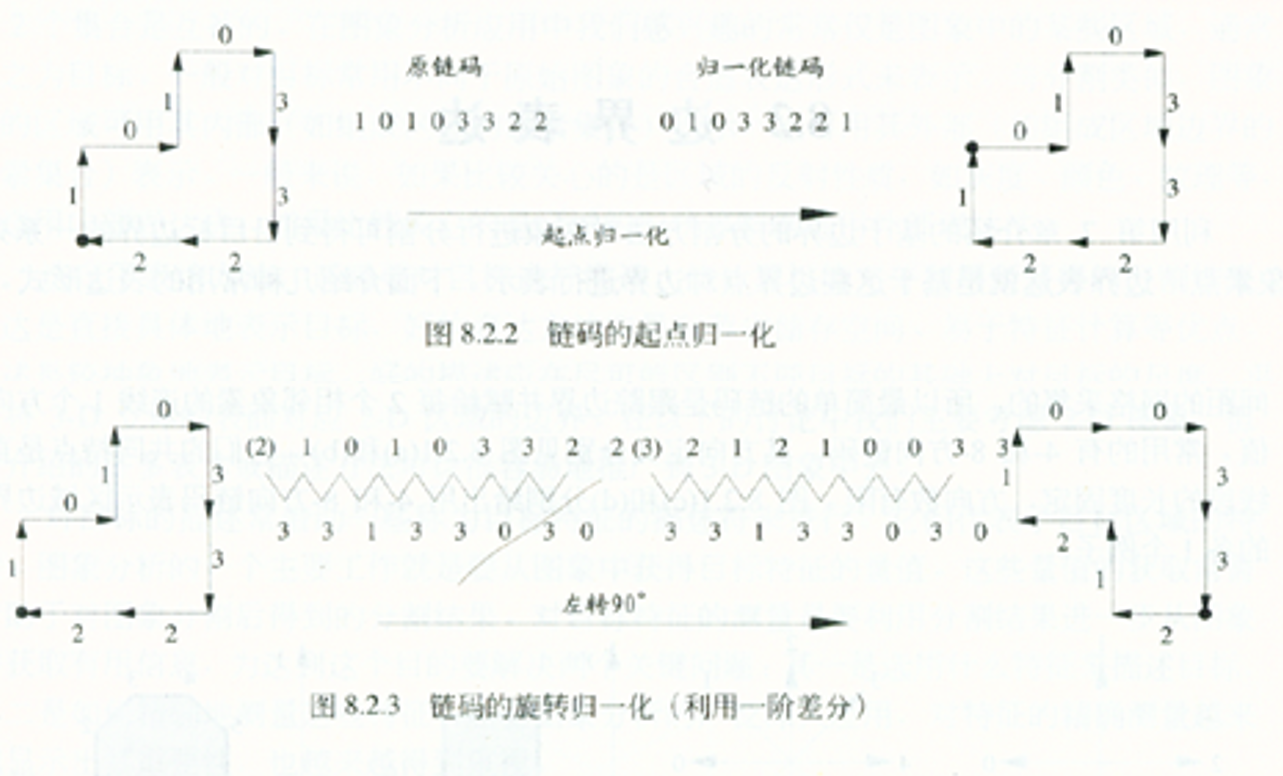
\includegraphics[width=0.8\linewidth]{fig/chain_code_difference.png}
\end{figure}

\subsubsection{多边形近似表达方法}
\begin{itemize}
	\item 基于收缩的最小周长多边形法:将原边界看作有弹性的线,在像素的约束下将线拉紧
	\item 基于聚合的最小均方误差线段逼近法:每个顶点到边的垂线距离小于$\delta$
	\item 基于分裂的最小均方误差线段逼近法
\begin{figure}[H]
\centering
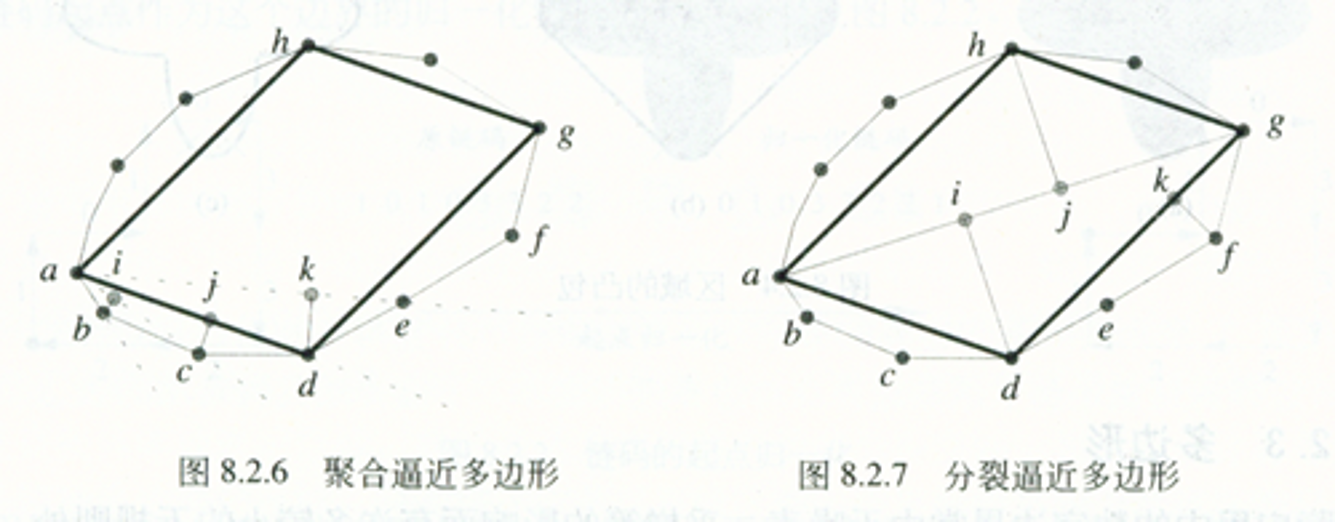
\includegraphics[width=0.8\linewidth]{fig/line_approx.png}
\end{figure}
\end{itemize}

基于收缩的最小周长多边形法(MPP算法):
围成一条数字边界的单元集合称为单元组合体。
令W、B分别表示凸顶点和镜像凹顶点的集合。
\begin{itemize}
	\item 由简单连接的单元组合体为边界的MPP是非自相交的。
	\item MPP的每个凸顶点都是一个W顶点,但并非边界的每个W顶点都是MPP的一个顶点。
	\item MPP的每个镜像凹顶点都是一个B顶点,但并非边界的每个B顶点都是MPP的一个顶点。
	\item 所有B顶点,要么在MPP上,要么在MPP外;
	所有W顶点,要么在MPP上,要么在MPP内
	\item 单元组合体包含的顶点序列的最左上角的顶点,总是MPP的一个W顶点。
\end{itemize}
\begin{figure}[H]
\centering
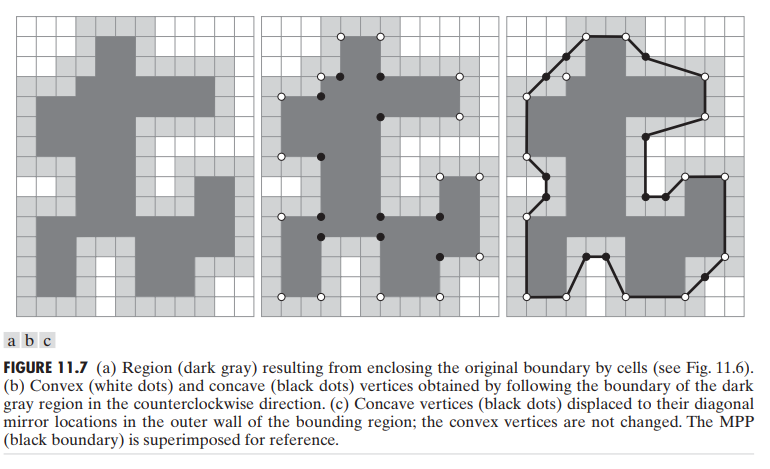
\includegraphics[width=0.8\linewidth]{fig/MPP.png}
\end{figure}

\subsubsection{标记图方法}
标记图是一种一维函数的边界表达方法
\begin{figure}[H]
\centering
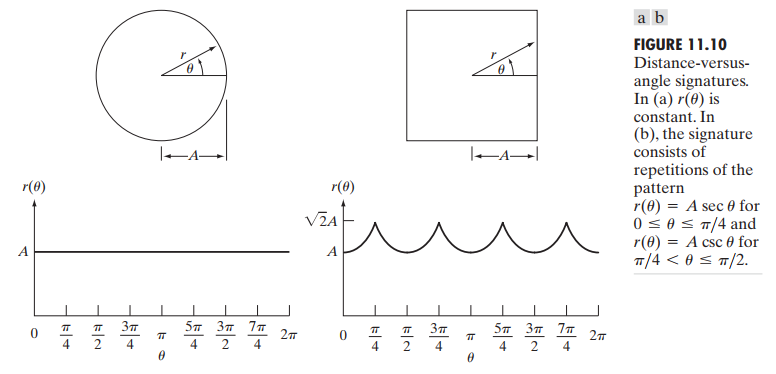
\includegraphics[width=0.8\linewidth]{fig/signature.png}
\end{figure}
\begin{itemize}
\item 不受目标平移影响,但受目标尺度变换和旋转的影响
\item 尺度变换影响可以通过将最大幅值归一化来解决
\item 旋转的影响解决方法
\begin{itemize}
	\item 选择离重心最远的点为标记起点
	\item 求出边界的主轴,以主轴上离重心最远的点作为标记起点
\end{itemize}
\end{itemize}

\subsubsection{边界线段}
将边界分段可以减小边界的复杂度。
\begin{figure}[H]
\centering
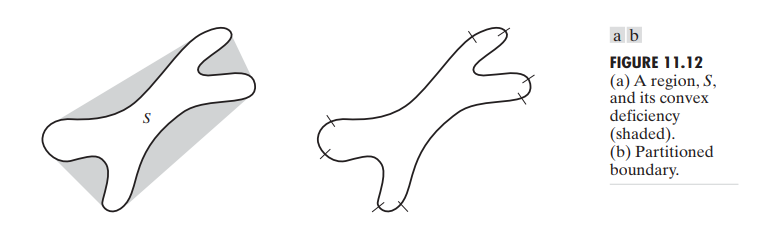
\includegraphics[width=0.8\linewidth]{fig/region_segmentation.png}
\end{figure}

\subsubsection{骨架}
表达平面区域结构形状的一种方法;
此方法可以用细化算法实现。
\begin{figure}[H]
\centering
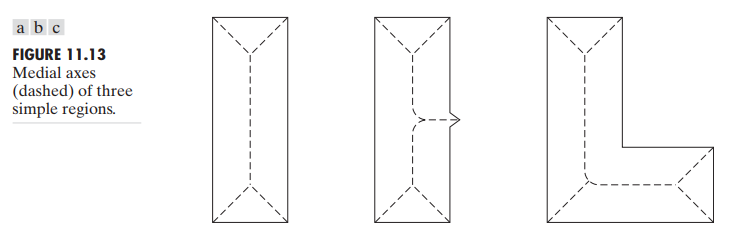
\includegraphics[width=0.8\linewidth]{fig/skeletons.png}
\end{figure}

集合$A$的骨架$S(A)$定义为
\[S(A)=\{z\mid A\text{内最大圆盘}(D)_z\text{的圆心}\}\]
\begin{figure}[H]
\centering
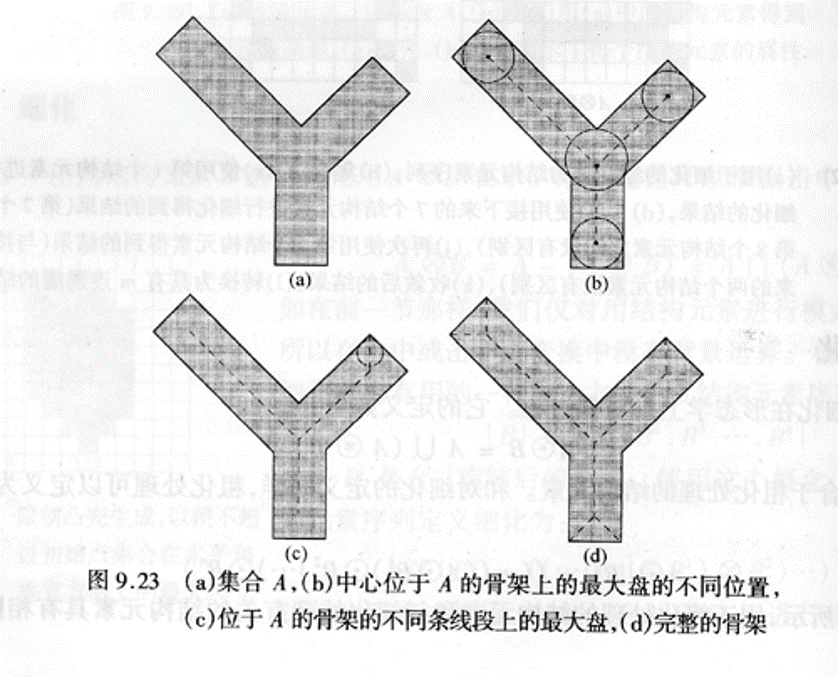
\includegraphics[width=0.6\linewidth]{fig/skeletons2.png}
\end{figure}

\subsection{边界描绘子}
\subsubsection{简单的描述符}
\begin{enumerate}
\item 边界的长度;
\item 边界的直径:边界上相隔最远两点的距离。($D$可以是任意距离度量)
\[Diam(B)=\max_{i,j}D(p_i,p_j),\;p_i\in B,p_j\in B\]
\item 曲率:斜率的变化率 。通常采用相邻边界线段的斜率差。
当沿顺时针方向沿着边界运动,当顶点$p$斜率变化量为非负的时候,称这一点属于凹线段;否则,称$p$属于凸线段。
\end{enumerate}

\subsubsection{形状数}
形状数是基于链码的一种边界形状描述符。
一个边界形状描述是其链码的差分码中值最小的一个序列。
形状数长度称为阶数。
\begin{figure}[H]
\centering
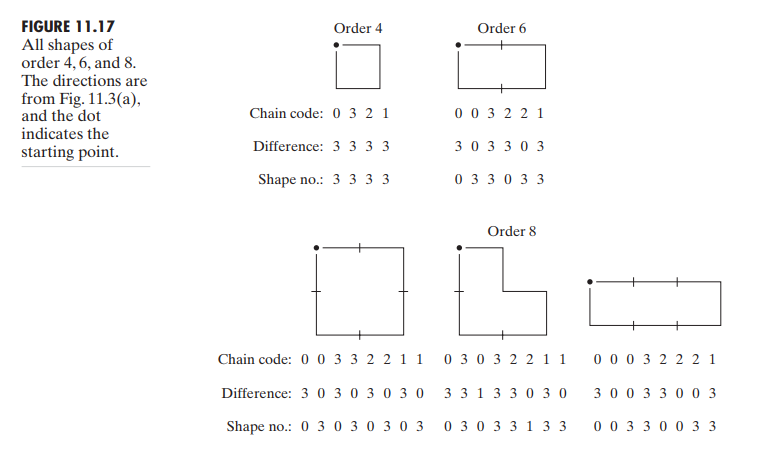
\includegraphics[width=0.8\linewidth]{fig/shape_number.png}
\end{figure}

\subsubsection{傅里叶描绘子}
将2D问题转化为1D问题,将边界点的坐标对表示成一个复数
\[s(k)=x(k)+jy(k),k=0,1,\ldots,k-1\]
对$s(k)$的傅氏变换为
\[a(u)=\frac{1}{K}\sum_{k=0}^{K-1}s(k)\ee^{-j2\pi uk/K},u=0,1,\ldots,K-1\]
复系数$a(u)$称为边界的描绘子。
\begin{figure}[H]
\centering
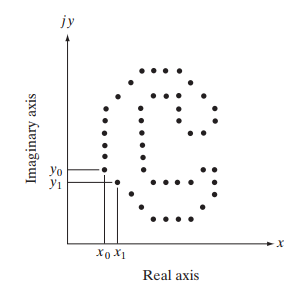
\includegraphics[width=0.3\linewidth]{fig/fourier_descriptor.png}
\end{figure}

傅氏反变换确定边界的重建:
\[s(k)=\sum_{u=0}^{K-1}a(u)\ee^{j2\pi uk/K},k=0,1,\ldots,K-1\]
通过有限重建构造近似边界
\[\hat{s}(k)=\sum_{u=0}^{p-1}a(u)\ee^{j2\pi uk/K},k=0,1,\ldots,K-1,K>P\]

\subsubsection{统计矩}
统计矩(statistical moment)用于刻画边界线段的特征波形。
\begin{figure}[H]
\centering
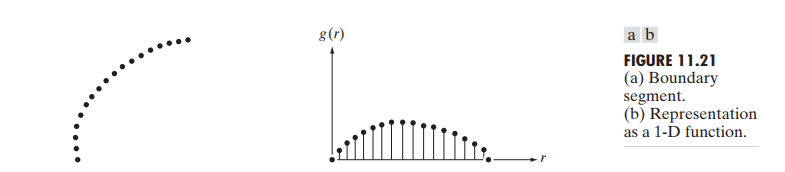
\includegraphics[width=0.8\linewidth]{fig/statistical_moment.png}
\end{figure}
\begin{enumerate}
	\item 将上述曲线看作一维函数$g(r)$
	\item 将$g$的振幅看作离散随机变量$v$,并形成直方图$p(v_i)$,其中$i=0,1,\ldots,A-1$
	\item 定义$n$阶中心矩
	\[\mu_n(v)=\sum_{i=0}^{A-1}(v_i-m)^np(v_i)\]
	其中$m=\sum_{i=0}^{A-1}v_ip(v_i)$,$m$是$v$的均值
\end{enumerate}

另一种统计矩:
\begin{enumerate}
	\item 将$g(r)$归一化为单位面积的函数,并作成直方图,即将$g(r_i)$作为产生值$r_i$的概率
	\item 定义$n$阶中心矩为
	\[\mu_n(r)=\sum_{i=0}^{K-1}(r_i-m)^ng(r_i)\]
	其中$m=\sum_{i=0}^{K-1}r_ig(r_i)$,$m$是$r$的均值
\end{enumerate}


\subsection{区域描绘子}
\subsubsection{简单的描述符}
\begin{enumerate}
\item 区域的面积:图象中对象区域的面积可以看作区域像素的总和。
通常关心一些不变量,如区域致密性:
\[(\text{周长})^2/\text{面积}\]

\item 区域的重心
\[\begin{cases}
\bar{x}=\frac{1}{A}\sum_{(x,y)\in\mathcal{R}}xf(x,y)\\
\bar{y}=\frac{1}{A}\sum_{(x,y)\in\mathcal{R}}yf(x,y)
\end{cases}\]
其中,$\mathcal{R}$代表一个区域,$A$代表区域面积。

\item 区域灰度/密度:
常用的区域灰度特征有目标灰度(或颜色分量)的最大值、最小值、中值、平均值、方差以及高阶矩等统计量。
\end{enumerate}

\subsubsection{拓扑描述符}
欧拉数
\[E=C-H\]
其中$C$为区域内连通组元数,$H$为区域内孔数。

将区域的网络进行目标区域的分类,可以分为顶点数$V$,边数$Q$,面数$F$,其欧拉公式为:
\[V-Q+F=C-H=E\]


\subsubsection{纹理}
\begin{itemize}
	\item 纹理就是由纹理基元按某种确定的规律或某种统计规律排列而成
	\item 纹理分为确定性纹理和随机性纹理
\end{itemize}

区域的纹理主要度量区域的平滑度、粗糙度和规律性。
描述纹理的方法主要有三种:统计方法、结构方法和频谱方法。
下文着重考虑统计方法。

区域灰度直方图的统计矩($n$阶中心矩):
\[\mu_n(z)=\sum_{i=0}^{L-1}(z_i-m)^np(z_i)\]
其中$p(z_i)$为归一化直方图

光滑度描述子
\[R=1-\frac{1}{1+\sigma^2(z)}\]
若$R=0$则表示平滑(区域平坦),$R=1$代表不平滑

其他度量
\begin{itemize}
	\item 一致性
	\[U=\sum_{i=0}^{L-1}p^2(z_i)\]
	\item 熵
	\[p=-\sum_{i=0}^{L-1}p(z_i)\log_2p(z_i)\]
\end{itemize}

共生矩阵:设$S$为目标区域$R$中具有特定空间联系的像素对的集合,则共生矩阵$G$可定义为:
\[G(g_1,g_2)=\#\{[(x_1,y_1),(x_2,y_2)]\in S\mid f(x_1,y_1)=g_1 \& f(x_2,y_2)=g_2\}\]

基于共生矩阵的描绘子
\[m_{x}=\sum_{i}^{K} i \sum_{j}^{K} p_{ij}, \quad m_{y}=\sum_{j}^{K} j \sum_{i}^{K} p_{ij}\]
\[\sigma_{x}^{2}=\sum_{i}^{K}\left(i-m_{x}\right)^{2} \sum_{j}^{K} p_{ij}, \quad \sigma_{y}^{2}=\sum_{j}^{K}\left(j-m_{y}\right)^{2} \sum_{i}^{K} p_{ij}\]
\[P(i)=\sum_{i}^{K} p_{ij}, \quad P(j)=\sum_{i}^{K} p_{ij}\]
\[m_{x}=\sum_{i}^{K} iP(i), \quad m_{y}=\sum_{i}^{R} jP(j)\]
\[\sigma_{x}^{2}=\sum_{i}^{K}\left(i-m_{x}\right)^{2} P(i), \quad \sigma_{y}^{2}=\sum_{j}^{R}\left(j-m_{y}\right)^{2} P(j)\]
\begin{itemize}
	\item 最大概率$\max_{i,j}(p_{ij})$
	\item 对比度(元素差异的$k$阶矩)
	\[\sum_i^K\sum_j^K(i-j)^kp_{ij}\]
	\item 同质性:$G$对角分布的紧密性
	\[\sum_i^K\sum_j^K \frac{p_{ij}}{1+|i-j|}\]
	\item 一致性:
	\[\sum_i^K\sum_j^K p_{ij}^2\]
	\item 熵:
	\[-\sum_i^K\sum_j^K p_{ij}\log_2 p_{ij}\]
	\item 相关性:
	\[\sum_i^K\sum_j^K\frac{(i-m_x)(j-m_y)p_{ij}}{\sigma_x\sigma_y}\]
\end{itemize}

二阶函数的矩:
对于二维连续函数$f(x,y)$,$(p+q)$-阶矩定义为
\[m_{pq}=\intabu{-\infty}{+\infty}{\intabu{-\infty}{+\infty}{x^py^qf(x,y)}{x}}{y}\]


\subsection{主分量描绘}
主分量分析(PCA)、Hotelling变化、特征变量变换、K-L变换

协方差矩阵
\[C_x=\E{(x-\bar{x})(x-\bar{x})^\T}\approx\frac{1}{L}\sum_{l=1}^Lx_lx_l^\T-\bar{x}\bar{x}^\T\]
其中$C_x$是半正定的实对称矩阵。

将图像堆积成\textbf{列}向量
\[\vx=\bmat{f(0,0), f(0,1), \ldots, f(0,N-1), f(1,0), f(1,1), \ldots, f(1,N-1), f(N-1,0), f(N-1,1), \ldots, f(N-1,N-1)}^\T\]

对$C_x$进行特征分析,得到一组实非负特征值$\lambda_1,\lambda_2,\ldots,\lambda_r$及对应的特征向量$V_1,V_2,\ldots,V_r$。

令$T=\bmat{V_1 & V_2 & \cdots & V_r}$,则$C_xT^\T=\bmat{\lambda_i}T^\T$,做变换$y=T(x-\bar{x})$,则
\[\begin{aligned}
C_y&=\E{yy^\T}=\E{T(x-\bar{x})(x-\bar{x})^\T T^\T}\\
&=T\E{(x-\bar{x})(x-\bar{x})^\T}T^\T\\
&=TC_xT^\T=T\bmat{\lambda_i}T^\T\\
&=\bmat{\lambda_i}=\bmat{\lambda_1 & \cdots & 0\\\cdots & \cdots & \cdots\\0 & \cdots & \lambda_N}
\end{aligned}\]
即$y$各元素互不相关,$T$为去相关变换,$\lambda_k$为变换后第$k$个分量$y_k$的方差。
任何向量$x$都可以通过$y$重构
\[x=T^\T y+\bar{x}\]

将特征根从大到小排列,记为$\lambda_1\geq\lambda_2\geq\cdots\geq\lambda_r$,同时将特征向量做相应排序,记为$V_1,V_2,\ldots,V_r$。
取$1<M<r$,使得$\sum_{i=1}^M\lambda_i\Big/\sum_{i=1}^r\lambda_i>\alpha$(如$\alpha=95\%$)

又令$T_M=\bmat{V_1 & V_2 & \cdots & V_M}^\T$,$\hat{y}=T_M(x-\bar{x})$,而$x$依然可以通过
\[\bar{x}=T^\T_M\hat{y}+\bar{x}\]
来近似重构,其均方误差为
\[\begin{aligned}
MSE &= \E{(x-\hat{x})^\T(x-\hat{x})}\\
&=\E{\lrp{\sum_{i=M+1}^r y_iV_i}^\T\lrp{\sum_{i=M+1}^ry_iV_i}}\\
&=\sum_{i=M+1}^r\E{y_i^2}\\
&=\sum_{i=M+1}^r\lambda_i
\end{aligned}\]

基于矩阵的奇异值分解(SVD),$\sqrt{\lambda_i}$为$A$的奇异值,有推论$u=Av\Lambda^{-1/2}$,即可取$AA^\T$与$A^\T A$中维数较小的矩阵计算特征向量。

可以将奇异值分解和PCA应用于多光谱图像的压缩。
% 关键看y=T(x-\bar{x}) 飞机图像